
%(BEGIN_QUESTION)
% Copyright 2006, Tony R. Kuphaldt, released under the Creative Commons Attribution License (v 1.0)
% This means you may do almost anything with this work of mine, so long as you give me proper credit

Den pneumatiske regulatoren Foxboro modell 43 brukte et buet, gjennomsiktig plastrør med en plastkule inni som ``null''-indikator for å hjelpe operatøren med å gjøre ``støtfrie'' overganger mellom auto- og manuell modus:

$$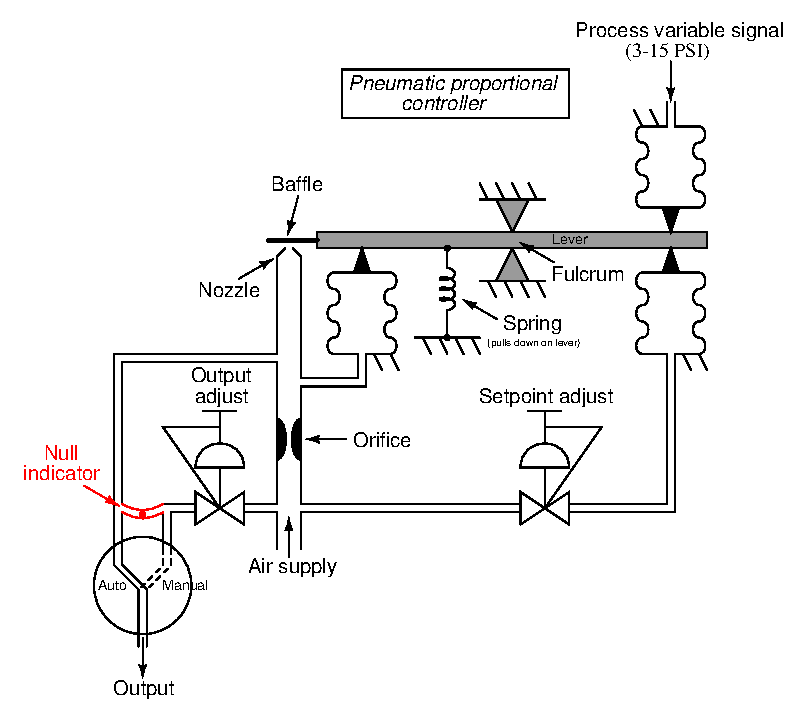
\includegraphics[width=15.5cm]{i01479x01.eps}$$

Lag en trinnvis instruksjon til en operatør for overgang fra auto til manuell modus, der denne nullindikatoren brukes for å sikre en jevn overgang mellom modusene.

\vskip 20pt \vbox{\hrule \hbox{\strut \vrule{} {\bf Forslag til sokratisk diskusjon} \vrule} \hrule}

\begin{itemize}
\item{} Forklar begrunnelsen for at en operatør bør gjøre en ``støtfri'' overgang med en regulator som denne.
\item{} Beskriv et realistisk reguleringsscenario der et ikke-støtfritt bytte mellom automatisk og manuell modus (eller omvendt) kan skape problemer for prosessen. Hvis det er nyttig, kan du vise til et P\&ID-diagram i lekser eller lærebok.
\item{} Anta at biasfjæren i mekanismen plutselig ryker. Forklar hvilke virkninger denne feilen vil ha på den pneumatiske regulatormekanismens funksjon.
\item{} Anta at regulatoren står i automatisk modus og indikatorskulen er helt til venstre. Beskriv nødvendige trinn for å bytte denne regulatoren til manuell modus på en ``støtfri'' måte.
\item{} Anta at regulatoren står i manuell modus og indikatorskulen er helt til venstre. Beskriv nødvendige trinn for å bytte denne regulatoren til automatisk modus på en ``støtfri'' måte.
\end{itemize}

\underbar{file i01479}
%(END_QUESTION)





%(BEGIN_ANSWER)

Tips: Kulen bør stå nøyaktig midt i røret før overføringsventilen flyttes.

%(END_ANSWER)





%(BEGIN_NOTES)

Trinn:

\begin{itemize}
\item{(1)} Juster ``Output Adjust''-regulatoren til kulen står i midten
\item{(2)} Flytt overføringsventilen fra ``Auto'' til ``Manual''.
\item{(3)} Juster ``Output Adjust''-regulatoren etter behov for manuell prosessregulering.
\end{itemize}



\vfil \eject

\noindent
{\bf Oppsummeringsquiz:}

Formålet med ``nullindikatoren'' i denne pneumatiske regulatoren er å:

$$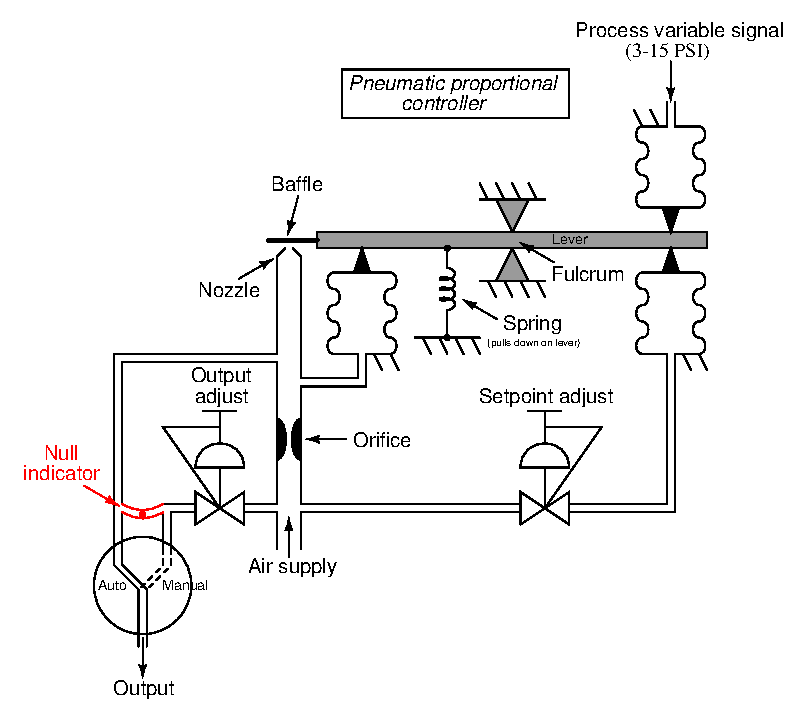
\includegraphics[width=15.5cm]{i01479x01.eps}$$

\begin{itemize}
\item{} Begrense hvor mye utgangssignaltrykk som sendes til reguleringsventilen
\vskip 5pt 
\item{} Dempe PV-signalet slik at regulatoren ikke påvirkes av støy
\vskip 5pt 
\item{} Gi operatøren en måte å få støtfri auto/manuell-overgang
\vskip 5pt 
\item{} Gi en enkel måte å justere regulatorens proporsjonalbånd på
\vskip 5pt 
\item{} Gi en praktisk indikasjon av regulatorens utgangssignaltrykk
\vskip 5pt 
\item{} Indikere når settpunktsignaltrykket og prosessvariabelsignalet er like
\end{itemize}


%INDEX% Control, proportional: bumpless output transfer (pneumatic)

%(END_NOTES)

